%!TEX root = ./main.tex

%\documentclass[11pt, a4paper, titlepage, slovak]{book}
\documentclass[12pt, a4paper, titlepage, slovak]{book}

%Includes all neccessary packets and contains some useful commands
%!TEX root = ./main.tex

% This file is part of the i10 thesis template developed and used by the
% Media Computing Group at RWTH Aachen University.
% The current version of this template can be obtained at
% <http://www.media.informatik.rwth-aachen.de/karrer.html>.



%-----------------------------------------------------------------------------------------------------------------------------------------
% Befehle
% commands
%-----------------------------------------------------------------------------------------------------------------------------------------

%----------------------------------------------------------------------------------
% \myBigFigure	[ LABEL_PREFIX (optional) ]
%				{ FILENAME (without extension) }
%				{ CAPTION TEXT }
%				{ SHORT VERSION OF CAPTION TEXT }
%
%Bild wird in kompletter Breite gesetzt, die Kurzversion der Bildunterschrift erscheint im Abbildungsverzeichnis
%picture using full width of the page, the short caption is what appears in the list of figures index

%----------------------------------------------------------------------------------
% \myFrameBigFigure	[ LABEL_PREFIX (optional) ]
%					{ FILENAME (without extension) }
%					{ CAPTION TEXT }
%					{ SHORT VERSION OF CAPTION TEXT }
%
%Bild wird in kompletter Breite gesetzt und eingerahmt, die Kurzversion der Bildunterschrift erscheint im Abbildungsverzeichnis
%picture with frame using the full width of the page, the short caption is what appears in the list of figures index

%----------------------------------------------------------------------------------
% \myHUGEFigure	[ LABEL_PREFIX (optional) ]
%				{ FILENAME (without extension) }
%				{ CAPTION TEXT }
%				{ SHORT VERSION OF CAPTION TEXT }
%
%Bild wird rotiert und quer in kompletter Breite gesetzt, die Kurzversion der Bildunterschrift erscheint im Abbildungsverzeichnis
%landscape picture using the full width of the rotated page, the short caption is what appears in the list of figures index

%----------------------------------------------------------------------------------
% \myFigure	[ LABEL_PREFIX (optional) ]
%			{ FILENAME (without extension) }
%			{ CAPTION TEXT }
%			{ SHORT VERSION OF CAPTION TEXT }
%
%Bild wird in der Breite der textspalte gesetzt, die Kurzversion der Bildunterschrift erscheint im Abbildungsverzeichnis
%picture using the width of the text column, the short caption is what appears in the list of figures index

%----------------------------------------------------------------------------------
% \myImgRef	[ LABEL_PREFIX (optional) ]
%			{ LABEL OF THE IMAGE }
%
%referenziert das angegebene Bild
%reference to an image

%----------------------------------------------------------------------------------
% \myBigTable	{ YOUR TABULAR DEFINITION }
%			{ CAPTION TEXT }
%			{ TABLE_LABLE }
%
%Tabelle wird in kompletter Breite gesetzt
%table using the full width of the page

%----------------------------------------------------------------------------------
% \myTable	{ YOUR TABULAR DEFINITION }
%			{ CAPTION TEXT }
%			{ TABLE_LABLE }
%
%Tabelle wird in der Breite der Textspalte gesetzt
%table using the width of the text column

%----------------------------------------------------------------------------------
% \myTxtRef	{ LABLE }
%
%Referenz auf Kapitel oder Abschnitte - gibt nummer und namen aus, z.B.: 5.3---"Yaddahyaddah"
%references chapters or sections, outputs number and title, e.g., 5.3---"Yaddahyaddah"

%----------------------------------------------------------------------------------
% \myUnderscore
%
%Setzt einen "schšnen" Unterstrich fŸr URLs
%typesets a 'nice' underscore for URLs

%----------------------------------------------------------------------------------
%\myTilde
%
%Setzt eine "schšne" Tilde fŸr URLs
%typesets a 'nice' tilde for URLs

%----------------------------------------------------------------------------------
% \myURL	{ TYPESET VERSION OF ANCHOR }
%			{ PRISTINE URL }
%			{ TYPESET VERSION OF URL }
%
%Setzt eine URL
%die typographisch "schšne" version erscheint in einer Fu§note,
%im Text erscheint der Ankertext, verlinkt ist die "echte" URL
%typesets a URL
%the typographically correct version appears as a footnote,
%the anchor appears in the text, the link points to the pristine URL

%----------------------------------------------------------------------------------
% \mySimpleURL	{ TYPESET VERSION OF ANCHOR }
%				{ PRISTINE URL }
%
%Setzt eine URL
%die URL erscheint in einer Fu§note,
%im Text erscheint der Ankertext, die URL ist verlinkt
%typesets a URL
%the URL appears as a footnote,
%the anchor appears in the text, the link points to the URL

%----------------------------------------------------------------------------------
% \myProjectURL	{ TYPESET VERSION OF ANCHOR }
%				{ PRISTINE URL INSIDE PROJECT DIRECTORY }
%				{ TYPESET VERSION OF URL INSIDE PROJECT DIRECTORY }
%
%Setzt eine URL innerhalb des Projektverzeichnisses auf "media"
%ACCOUNT muss durch den eigenen Usernamen ersetzt werden
%die typographisch "schšne" version erscheint in einer Fu§note,
%im Text erscheint der Ankertext, verlinkt ist die "echte" URL
%typesets a URL inside the project directory on 'media'
%replace ACCOUNT with your username
%the typographically correct version appears as a footnote,
%the anchor appears in the text, the link points to the pristine URL

%----------------------------------------------------------------------------------
% \mnote	{ MARGIN NOTE }
%
%Setzt eine Randnotitz
%puts a comment into the margin in small sans-serif font

%----------------------------------------------------------------------------------
% \todo	{ TODO MARGIN NOTE }
%
%Setzt eine "ToDo"-Randnotitz in rot zur Erinnerung
%puts a 'todo' comment into the margin in red

%----------------------------------------------------------------------------------
% \chapterquote	{ QUOTATION }
%				{ SOURCE }
%
%Setzt ein Zitat zum Einleiten eines Kapitels
%outputs a quote with its source, can be used as an introduction to chapters

%----------------------------------------------------------------------------------
% \myDefBox	{ TERM }
%			{ DEFINITION }
%
%Setzt eine Randnotitz und eine farbige Box (Textspaltenbreite),
%welche einen Begriff und seine Definition enthŠlt
%outputs a margin note and a colored box (width of the text column) containing a term and its definition

%----------------------------------------------------------------------------------
% \myBigDefBox	{ TERM }
%				{ DEFINITION }
%
%Setzt eine farbige Box (Seitenbreite), welche einen Begriff und seine Definition enthŠlt
%outputs a colored box (width of the page) containing a term and its definition

%----------------------------------------------------------------------------------
% \myDownloadURL	{ TYPESET DOWNLOAD NAME }
%					{ PRISTINE VERSION OF FILENAME }
%					{ TYPESET VERSION OF FILENAME }
%
%Setzt eine farbige Box, welche einen Downloadlink enthŠlt
%outputs a colored box containing a download link

%----------------------------------------------------------------------------------
% \emptydoublepage
%
% Leere Doppelseite ohne Kopf- oder Fu§zeile am Ende von Kapiteln
% Clear double page without any header or footer at end of chapters

%----------------------------------------------------------------------------------
% \pagebreak	[ SOME STRANGE LATEX VALUE ]
%
%Eklige pagebreaks fŸr den Druck (falls es nicht mehr anders geht)
%pagebreaks for the final print version (last resort weapon against wrong pagebreaks by LaTeX)

%----------------------------------------------------------------------------------
% \TM
%
%Setzt ein (TM) Symbol
%Places a (TM) symbol


%----------------------------------------------------------------------------------
%Packages and parameters
%----------------------------------------------------------------------------------

%inputencoding for the mac
\usepackage[utf8]{inputenc}
\usepackage[slovak,english]{babel}

%packages for mathematical symbols
\usepackage{latexsym}
\usepackage{amsmath}
\usepackage{amssymb}

% removes 'chapter' word from titles and apply own style
\usepackage{titlesec}
\titleformat{\chapter}{\normalfont\huge\bf}{\thechapter.}{20pt}{\huge\bf}

%table design
\usepackage{booktabs}

%grahics package
\usepackage{color,graphicx}

%path to your image folder
\graphicspath{{images/}}

%do not indent at new paragraphs but add a vertical offset
\usepackage{noindent}

%change standard fonts to Palatino and Helvetica
\usepackage{helvet}

%bibliography settings
\usepackage{natbib}
\bibliographystyle{apalike}

%source code listings
\usepackage{color}
\usepackage{xcolor}
\usepackage{listings}
\usepackage{caption}
\DeclareCaptionFont{white}{\color{white}}
\DeclareCaptionFormat{listing}{\colorbox{gray}{\parbox{\textwidth}{#1#2#3}}}
\captionsetup[lstlisting]{format=listing,labelfont=white,textfont=white}
\renewcommand{\lstlistingname}{Algoritmus}

%highlits
\usepackage{framed}
\definecolor{shadecolor}{rgb}{0.75,0.75,0.75}

%citation commands
\newcommand{\fullcite}{\citep} %for "Author [1980]"
\renewcommand{\citeyear}{\citeyearpar} %for "[1980]"

\usepackage{setspace}
%\doublespacing
\onehalfspacing


%package for control structures
\usepackage{ifthen}

%marginpar hack --- moves margin notes to correct position
\usepackage{mparhack}

%make readable references
\usepackage[pdftex,plainpages=false,pdfpagelabels]{hyperref}


%---------------------<Layout in the style of "A Pattern Approach to Interaction Design>---------------------------

% Change page headers and footers:
\usepackage{fancyhdr}
\pagestyle{fancy}
\fancyhf{}
\fancyhead[RE]{\slshape \nouppercase{\leftmark}}    % Even page header: "page   chapter"
\fancyhead[LO]{\slshape \nouppercase{\rightmark}}   % Odd  page header: "section   page"
\fancyhead[RO,LE]{\bfseries \thepage} 
\renewcommand{\headrulewidth}{1pt}    % Underline headers
\renewcommand{\footrulewidth}{0pt}    

\fancypagestyle{plain}{               % No chapter+section on chapter start pages
\fancyhf{}
\fancyhead[RO,LE]{\bfseries \thepage}
\renewcommand{\headrulewidth}{1pt}
\renewcommand{\footrulewidth}{0pt}
}

% Left headings: "1  INTRODUCTION"
\renewcommand{\chaptermark}[1]{%
\markboth{\thechapter\ \ \ \ #1}{}}

% Right headings: "1.1  Basics"
\renewcommand{\sectionmark}[1]{%
\markright{\thesection\ \ \ \ #1}{}}

% some Fancyhdr problem...
\addtolength{\headheight}{2pt} % To avoid overfull vboxes from fancyhdr

%creating a better way to change the layout for the abstract pages
\usepackage{geometry}

\titlespacing*{\chapter}{0pt}{0pt}{25pt}

\ifthenelse{\lengthtest{\paperheight=250mm}}%
{% -----------------B5 Layout-----------------
% Page layout

%\pdfpageheight250mm
%\pdfpagewidth176mm
\geometry{	b5paper,
			top = 27mm,
			footskip = 10mm,
			inner = 19mm,
			outer = 39mm,
			textheight = 175mm,
			textwidth = 84mm,
			marginparsep = 3mm,
			marginparwidth = 32mm
}
\savegeometry{myText}
% -----------------/ B5 Layout-----------------
}%
{% -----------------A4 Layout-----------------
% Page layout
\geometry{	a4paper,
			twoside,
			includemp,
			includehead,
			top = 20mm,
			headsep = 10mm,
			bindingoffset = 0mm,
			inner = 40mm,
			outer = 30mm,
			bottom = 30mm,
			marginparsep = 0mm,
			marginparwidth = 0mm
}
\savegeometry{myText}
% -----------------/ A4 Layout-----------------
}
% Abstract layout
\geometry{	marginparsep = 0mm,
			marginparwidth = 0mm
}
\savegeometry{myAbstract}
\loadgeometry{myText}


\newlength{\fullwidth} % Width of text plus margin notes
\setlength{\fullwidth}{\textwidth}
\addtolength{\fullwidth}{\marginparsep}
\addtolength{\fullwidth}{\marginparwidth}

\setlength{\headwidth}{\fullwidth} % Header stretches over margin notes


%---------------------</Layout in the style of "A Pattern Approach to Interaction Design>---------------------------


%wird fŸr die flŠchendeckende Ausgabe der Titelseite benštigt
%needed for the full-face titlepage
\usepackage{eso-pic}

%index verwenden
%make an index
\usepackage{makeidx}
\makeindex

%Index Formatierungshilfen
%formatting helpers for the index
\newcommand{\uu}[1]{\underline{#1}}
\newcommand{\ii}[1]{\textit{#1}}

%neue Definition der Index Umgebung
%redesign of the index
\renewenvironment{theindex}{%
  \vspace*{50pt}%
  {\Huge\bfseries\indexname}\par%
  \vspace*{40pt}%
  \setlength{\parskip}{0pt}%
  \setlength{\parindent}{0pt}%
  \small%
  \renewcommand{\item}{\par{}}%
  \renewcommand{\subitem}{\par\hspace{2em}- }%
}%
{}

%Maximale Gliederungstiefe, die noch ins Inhaltsverzeichnis aufgenommen wird
%maximum depth for the table of contents
\setcounter{tocdepth}{3}

%Vorschlag fŸr ein schšnes Farbschema
%Set of colors which look nice together
\usepackage{color}
\definecolor{orange_light}{rgb}{1,0.8,0.4}
\definecolor{orange_med}{rgb}{0.753,0.62,0.373}
\definecolor{orange_dark}{rgb}{0.506,0.412,0.251}

\definecolor{green_light}{rgb}{0.8,1,0.4}
\definecolor{green_med}{rgb}{0.635,0.745,0.376}
\definecolor{green_dark}{rgb}{0.435,0.498,0.255}

\definecolor{blue_light}{rgb}{0.4,0.8,1}
\definecolor{blue_med}{rgb}{0.365,0.624,0.749}
\definecolor{blue_dark}{rgb}{0.251,0.42,0.502}

\definecolor{pink_light}{rgb}{1,0.435,0.812}
\definecolor{pink_med}{rgb}{0.745,0.38,0.62}
\definecolor{pink_dark}{rgb}{0.498,0.255,0.416}

\definecolor{yellow_light}{rgb}{1,1,0.4}
\definecolor{yellow_med}{rgb}{0.757,0.745,0.373}
\definecolor{yellow_dark}{rgb}{0.506,0.49,0.251}

%blau (fŸr URLs)
%blue (for URLs)
\definecolor{blue}{rgb}{0,0,1}

%notwendig fŸr die korrekte Erkennung, auf welcher Seite sich eine Abbildung befindet.
%we need this to determine if a figure is on an odd or even page
\usepackage{chngpage}

%Hiermit kšnnen die Abbildungslegenden frei gestaltet werden
%we need this to redesign the captions
\usepackage[font=normalsize,labelfont=bf]{caption}

%Abbildungen kommen auf eine eigene Seite, wenn sie mehr als 85% des Platzes
%auf einer Seite einnehmen
%if a figure takes more than 85% of a page it will be typeset on a separate page
\renewcommand{\floatpagefraction}{0.85}

%Benštigt um gro§e Abbildungen gedreht auf eine Seite zu setzen
%we need this to rotate big figures
\usepackage[figuresright]{rotating}

%Verschiedene LŠngenma§e fŸr Textboxen
%dimensions for textboxes
\newlength{\myDefBoxWidth}
\setlength{\myDefBoxWidth}{\textwidth}
\addtolength{\myDefBoxWidth}{-4mm}
\newlength{\myBigDefBoxWidth}
\setlength{\myBigDefBoxWidth}{\fullwidth}
\addtolength{\myBigDefBoxWidth}{-4mm}

%Formathilfen fŸr MatLab Code (wer's braucht...)
%pre-defined matlab code formats
\usepackage{alltt}
\definecolor{string}{rgb}{0.7,0.0,0.0}
\definecolor{comment}{rgb}{0.13,0.54,0.13}
\definecolor{keyword}{rgb}{0.0,0.0,1.0}



%-----------------------------------------------------------------------------------------------------------------------------------------
% neue Befehle
% new commands
%-----------------------------------------------------------------------------------------------------------------------------------------

%----------------------------------------------------------------------------------
\renewcommand{\figurename}{Obrázok}

% \myBigFigure	[ LABEL_PREFIX (optional) ]
%				{ FILENAME (without extension) }
%				{ CAPTION TEXT }
%				{ SHORT VERSION OF CAPTION TEXT }
%
%Bild wird in kompletter Breite gesetzt
%picture using full width of the page
\newcommand{\myBigFigure}[4][image]
{%
\begin{figure}[t!bp]%
	\checkoddpage%
	\ifcpoddpage%
		%nothing
	\else
		\hspace{-\marginparsep}\hspace{-\marginparwidth}%
	\fi
	%use minipage to center the label beneath the figure
	\begin{minipage}{\fullwidth}%
		\includegraphics[width= \fullwidth]{#2}%
		\caption[#4]{#3}%
		\label{#1_#2}%
	\end{minipage}%
\end{figure}%
}


%----------------------------------------------------------------------------------
% \myFrameBigFigure	[ LABEL_PREFIX (optional) ]
%					{ FILENAME (without extension) }
%					{ CAPTION TEXT }
%					{ SHORT VERSION OF CAPTION TEXT }
%
%Bild wird in kompletter Breite gesetzt und eingerahmt
%picture with frame using the full width of the page
\newcommand{\myFrameBigFigure}[4][image]
{
\begin{figure}[t!bp]
	\checkoddpage
	\ifcpoddpage
		%nothing
	\else
		\hspace{-\marginparsep}\hspace{-\marginparwidth}
	\fi
	%use minipage to center the label beneath the figure
	\begin{minipage}{\fullwidth}
	\frame{%
		\includegraphics[width= \fullwidth]{#2}%
		}
		\caption[#4]{#3}
		\label{#1_#2}
	\end{minipage}
\end{figure}
}

%----------------------------------------------------------------------------------
% \myHUGEFigure	[ LABEL_PREFIX (optional) ]
%				{ FILENAME (without extension) }
%				{ CAPTION TEXT }
%				{ SHORT VERSION OF CAPTION TEXT }
%
%Bild wird rotiert und quer in kompletter Breite gesetzt
%landscape picture using the full width of the rotated page
\newcommand{\myHugeFigure}[4][image]
{
\begin{sidewaysfigure}[t!bp]
	\checkoddpage
	\ifcpoddpage
		%nothing
		\vspace{\marginparsep}\vspace{\marginparwidth}
	\else
		%nothing
		\vspace{-\marginparsep}\vspace{-\marginparwidth}
	\fi
		\includegraphics[width= \textheight]{#2}
		\caption[#4]{#3}
		\label{#1_#2}
	
\end{sidewaysfigure}
}

%----------------------------------------------------------------------------------
% \myFigure	[ LABEL_PREFIX (optional) ]
%			{ FILENAME (without extension) }
%			{ CAPTION TEXT }
%			{ SHORT VERSION OF CAPTION TEXT }
%
%Bild wird in der Breite der textspalte gesetzt
%picture using the width of the text column
\newcommand{\myFigure}[4][image]%
{%
\begin{figure}[t!bp]%
	\begin{center}%
		\includegraphics[width= \textwidth]{#2}%
		\caption[#4]{#3}
		\label{#1_#2}%
	\end{center}%
\end{figure}%
}%

%----------------------------------------------------------------------------------
% \myImgRef	[ LABEL_PREFIX (optional) ]
%			{ LABEL OF THE IMAGE }
%
%referenziert das angegebene Bild
%reference to an image
\newcommand{\myImgRef}[2][image]%
{%
	\ref{#1_#2}%
}%

%----------------------------------------------------------------------------------
% \myBigTable	{ YOUR TABULAR DEFINITION }
%			{ CAPTION TEXT }
%			{ TABLE_LABLE }
%
%Tabelle wird in kompletter Breite gesetzt
%table using the full width of the page
\newcommand{\myBigTable}[3]%
{%
\begin{table}[htdp]%
	\checkoddpage%
	\ifcpoddpage%
		%nothing
	\else%
		\hspace{-\marginparsep}\hspace{-\marginparwidth}%
	\fi%
	\begin{minipage}{\fullwidth}%
		\begin{center}%
			#1%
			\caption{#2}%
			\label{#3}%
		\end{center}%	
	\end{minipage}%
\end{table}%
}%

%----------------------------------------------------------------------------------
% \myTable	{ YOUR TABULAR DEFINITION }
%			{ CAPTION TEXT }
%			{ TABLE_LABLE }
%
%Tabelle wird in der Breite der Textspalte gesetzt
%table using the width of the text column
\newcommand{\myTable}[3]%
{%
\begin{table}[htdp]%
	\begin{center}%
		#1%
		\caption{#2}%
		\label{#3}%
	\end{center}%	
\end{table}%
}%

%----------------------------------------------------------------------------------
% \myTxtRef	{ LABLE }
%
%Referenz auf Kapitel oder Abschnitte - gibt nummer und namen aus, z.B.: 5.3---"Yaddahyaddah"
%references chapters or sections, outputs number and title, e.g., 5.3---"Yaddahyaddah"
\newcommand{\myTxtRef}[1]
{%
	\ref{#1} ``\nameref{#1}''%
}

%----------------------------------------------------------------------------------
% \myTxtRefPP	{ LABLE }
%
%Referenz auf Kapitel oder Abschnitte - gibt nummer, namen und seiten aus, z.B.: 5.3---"Yaddahyaddah" (p. 45)
%references chapters or sections, outputs number and title, e.g., 5.3---"Yaddahyaddah"
\newcommand{\myTxtRefPP}[1]
{%
	\ref{#1} ``\nameref{#1}'' (p.~\pageref{#1})%
}

%----------------------------------------------------------------------------------
% \myUnderscore
%
%Setzt einen "schšnen" Unterstrich fŸr URLs
%typesets a 'nice' underscore for URLs
\newcommand{\myUnderscore}{$\underline{\hspace{0.5em}}$}

%----------------------------------------------------------------------------------
%\myTilde
%
%Setzt eine "schšne" Tilde fŸr URLs
%typesets a 'nice' tilde for URLs
\newcommand{\myTilde}{$\sim$}

%----------------------------------------------------------------------------------
% \myURL	{ TYPESET VERSION OF ANCHOR }
%			{ PRISTINE URL }
%			{ TYPESET VERSION OF URL }
%
%Setzt eine URL
%die typographisch "schšne" version erscheint in einer Fu§note,
%im Text erscheint der Ankertext, verlinkt ist die "echte" URL
%typesets a URL
%the typographically correct version appears as a footnote,
%the anchor appears in the text, the link points to the pristine URL
\newcommand{\myURL}[3]%
{%
	\textcolor{blue}{%
		\href{#2}{#1}%
	}%
	\footnote{#3}%
}

%----------------------------------------------------------------------------------
% \mySimpleURL	{ TYPESET VERSION OF ANCHOR }
%				{ PRISTINE URL }
%
%Setzt eine URL
%die URL erscheint in einer Fu§note,
%im Text erscheint der Ankertext, die URL ist verlinkt
%typesets a URL
%the URL appears as a footnote,
%the anchor appears in the text, the link points to the URL
\newcommand{\mySimpleURL}[2]%
{%
	\textcolor{blue}{%
		\href{#2}{#1}%
	}%
	\footnote{#2}%
}

%----------------------------------------------------------------------------------
% \myProjectURL	{ TYPESET VERSION OF ANCHOR }
%				{ PRISTINE URL INSIDE PROJECT DIRECTORY }
%				{ TYPESET VERSION OF URL INSIDE PROJECT DIRECTORY }
%
%Setzt eine URL auf hci/public wo die Inhalte des WebServer Ordners auf "oliver" verfŸgbar sind
%die typographisch "schšne" version erscheint in einer Fu§note,
%im Text erscheint der Ankertext, verlinkt ist die "echte" URL
%typesets a URL to hci/public from where the contents of the WebServer folder from oliver can be accessed
%the typographically correct version appears as a footnote,
%the anchor appears in the text, the link points to the pristine URL
\newcommand{\myProjectURL}[3]%
{%
	\textcolor{blue}{%
		\href{http://hci.rwth-aachen.de/public/#2}{#1}%
	}%
	\footnote{http://hci.rwth-aachen.de/public/#3}%
}

%----------------------------------------------------------------------------------
% \mnote	{ MARGIN NOTE }
%
%Setzt eine Randnotitz
%puts a comment into the margin in small sans-serif font
\newcommand{\mnote}[1]%
{%
	\leavevmode%
	\checkoddpage%
	\ifcpoddpage%
		\marginpar{\raggedright\textsf{{\footnotesize{#1}}}}%
	\else%
		\marginpar{\raggedleft\textsf{{\footnotesize{#1}}}}%
	\fi%
}
	
% leavevmode allows mnotes to be aligned with the first line of a paragraph
% NOTE: you have to put a "%" at the end of the line with the mnote, or you will get an extra blank at the beginning of the paragraph!

%----------------------------------------------------------------------------------
% \todo	{ TODO MARGIN NOTE }
%
%Setzt eine "ToDo"-Randnotitz in rot zur Erinnerung
%puts a 'todo' comment into the margin in red
\definecolor{red}{rgb}{1,0,0}
\newcommand{\todo}[1]{\mnote{\textcolor{red}{ToDo: #1}}}

%----------------------------------------------------------------------------------
% \chapterquote	{ QUOTATION }
%				{ SOURCE }
%
%Setzt ein Zitat zum Einleiten eines Kapitels
%outputs a quote with its source, can be used as an introduction to chapters
\newcommand{\chapterquote}[2]{
\begin{quotation}
    \begin{flushright}
	\noindent\emph{``{#1}''\\[1.5ex]---{#2}}
    \end{flushright}
\end{quotation}
}

%----------------------------------------------------------------------------------
% \myDefBox	{ TERM }
%			{ DEFINITION }
%
%Setzt eine Randnotitz und eine farbige Box (Textspaltenbreite),
%welche einen Begriff und seine Definition enthŠlt
%outputs a margin note and a colored box (width of the text column) containing a term and its definition
\newcommand{\myDefBox}[2]
{%
	\setlength{\fboxrule}{1mm}%
	\fcolorbox{orange_med}{orange_light}%
	{%
		\parbox{\myDefBoxWidth}{{\bfseries\scshape#1:}\\#2}%
	}%
	\mnote{Definition:\\\emph{#1}}
}

%----------------------------------------------------------------------------------
% \myBigDefBox	{ TERM }
%				{ DEFINITION }
%
%Setzt eine farbige Box (Seitenbreite), welche einen Begriff und seine Definition enthŠlt
%outputs a colored box (width of the page) containing a term and its definition
\newcommand{\myBigDefBox}[2]
{%
	\begin{figure}[h!]
	\setlength{\fboxrule}{1mm}%
	\checkoddpage%
	\ifcpoddpage%
		%nothing
	\else%
		\hspace{-\marginparsep}\hspace{-\marginparwidth}%
	\fi%
	\fcolorbox{orange_med}{orange_light}%
	{%
		\parbox{\myBigDefBoxWidth}{{\bfseries\scshape#1:}\\#2}%
	}%
	\end{figure}
}

%----------------------------------------------------------------------------------
% \myDownloadURL	{ TYPESET DOWNLOAD NAME }
%					{ PRISTINE VERSION OF FILENAME }
%					{ TYPESET VERSION OF FILENAME }
%
%Setzt eine farbige Box, welche einen Downloadlink enthŠlt
%outputs a colored box containing a download link
\newcommand{\myDownloadURL}[3]{%
\checkoddpage%
	\ifcpoddpage%
		%nothing
	\else%
		\hspace{-\marginparsep}\hspace{-\marginparwidth}%
	\fi%
\setlength{\fboxrule}{1mm}%
\fcolorbox{green_med}{green_light}{%
\begin{minipage}{\myBigDefBoxWidth}%
\begin{center}%
\myProjectURL{#1}{folder/#2}{folder/#3}%
\end{center}%
\end{minipage}%
}%
}

%----------------------------------------------------------------------------------
% \emptydoublepage
%
% Leere Doppelseite ohne Kopf- oder Fu§zeile am Ende von Kapiteln
% Clear double page without any header or footer at end of chapters
\newcommand{\emptydoublepage}{\clearpage\thispagestyle{empty}\cleardoublepage}

%----------------------------------------------------------------------------------
% \pagebreak	[ SOME STRANGE LATEX VALUE ]
%
%Eklige pagebreaks fŸr den Druck (falls es nicht mehr anders geht)
%pagebreaks for the final print version (last resort weapon against wrong pagebreaks by LaTeX)
\newcommand{\PB}[1][3]
{%
	\pagebreak[#1]%
}

%----------------------------------------------------------------------------------
% \TM
%
%Setzt ein (TM) Symbol
%Places a (TM) symbol
\newcommand{\TM}
{%
	\textsuperscript{\texttrademark}%
}


% zalamovanie slov
\hyphenation{
Twitter
Twittru
map-reduce
oblastiach
korpusov
processing
modelu
vstupno
ZeroMQ
tieto
priamo
vtedy
}


%--------------------------------------------------------------
\begin{document}

% allow more flexible whitespaces to avoid hyphenation and overfull hboxes
\sloppy %lepsi algoritmus na zalamovanie riadkov

% 'see'-entries for the index
%!TEX root = ./main.tex
%
% This file is part of the i10 thesis template developed and used by the
% Media Computing Group at RWTH Aachen University.
% The current version of this template can be obtained at
% <http://www.media.informatik.rwth-aachen.de/karrer.html>.

\index{abbrv|see{abbreviation}}




%--------------------------------------------------------------
% uvodne strany... obal, titulka, abstrakt, uvod, ...
%--------------------------------------------------------------
\frontmatter

%use the titlepage from the 'images' directory 
\newgeometry{rmargin=20mm}
\begin{titlepage}
% centrovanie
\begin{center}                                                                                                                                                   
{\Large Slovenská technická univerzita v Bratislave} \\
{\Large Fakulta informatiky a informačných technológií} \\
\vspace*{1\baselineskip}
\large {FIIT-5212-8279}
\vfill % vert. plnenie prazdnymi medzerami                                                                                                                                                                    

%\newpage

{{Matúš Cimerman}} \\
\vspace*{1\baselineskip}
{\huge {\textbf{Analýza prúdu údajov}}} % nadpis
%{\huge {Analýza prúdu údajov}} % nadpis
\\
\vspace*{1\baselineskip}
%{\Large {Bakalárska práca}}\\
\textit{Bakalárska práca}\\
\vfill %vert. plnenie
\end{center}
% end centrovanie
{Vedúci práce: Ing. Jakub Ševcech}\\
\\
%\vspace*{1\baselineskip}
{máj, 2015}
\end{titlepage}
\emptydoublepage

\begin{titlepage}
% centrovanie
\begin{center}                                                                                                                                                   
{\Large Slovenská technická univerzita v Bratislave} \\
{\Large Fakulta informatiky a informačných technológií} \\
\vspace*{1\baselineskip}
\large {FIIT-5212-8279}
\vfill % vert. plnenie prazdnymi medzerami                                                                                                                                                                    


{{Matúš Cimerman}} \\
\vspace*{1\baselineskip}
{\huge {\textbf{Analýza prúdu údajov}}} % nadpis
%{\huge {Analýza prúdu údajov}} % nadpis
\\
\vspace*{1\baselineskip}
%{\Large {Bakalárska práca}}\\
\textit{Bakalárska práca}\\
\vfill %vert. plnenie
\end{center}
% end centrovanie
{Študijný program: Informatika}\\
{Študijný odbor: 9.2.1 Informatika}\\
{Miesto vypracovania: Ústav informatiky a softvérového inžinierstva, FIIT STU Bratislava}\\
{Vedúci práce: Ing. Jakub Ševcech}\\
\\
{máj, 2015}

\end{titlepage}
\restoregeometry
\thispagestyle{empty}
\emptydoublepage

%% This file is part of the i10 thesis template developed and used by the
% Media Computing Group at RWTH Aachen University.
% The current version of this template can be obtained at
% <http://www.media.informatik.rwth-aachen.de/karrer.html>.

~
\vfill
I hereby declare that I have created this work completely on my own and used no other sources or tools than the ones listed, and that I have marked any citations accordingly.

\begin{flushright}
\vspace{12mm}
$\overline{Bratislava, MONTH \mathit{YEAR}}$\\
\textit{YOUR NAME}
\end{flushright}

%\emptydoublepage

%pred abstrakt treba vlozit jebnute zadanie
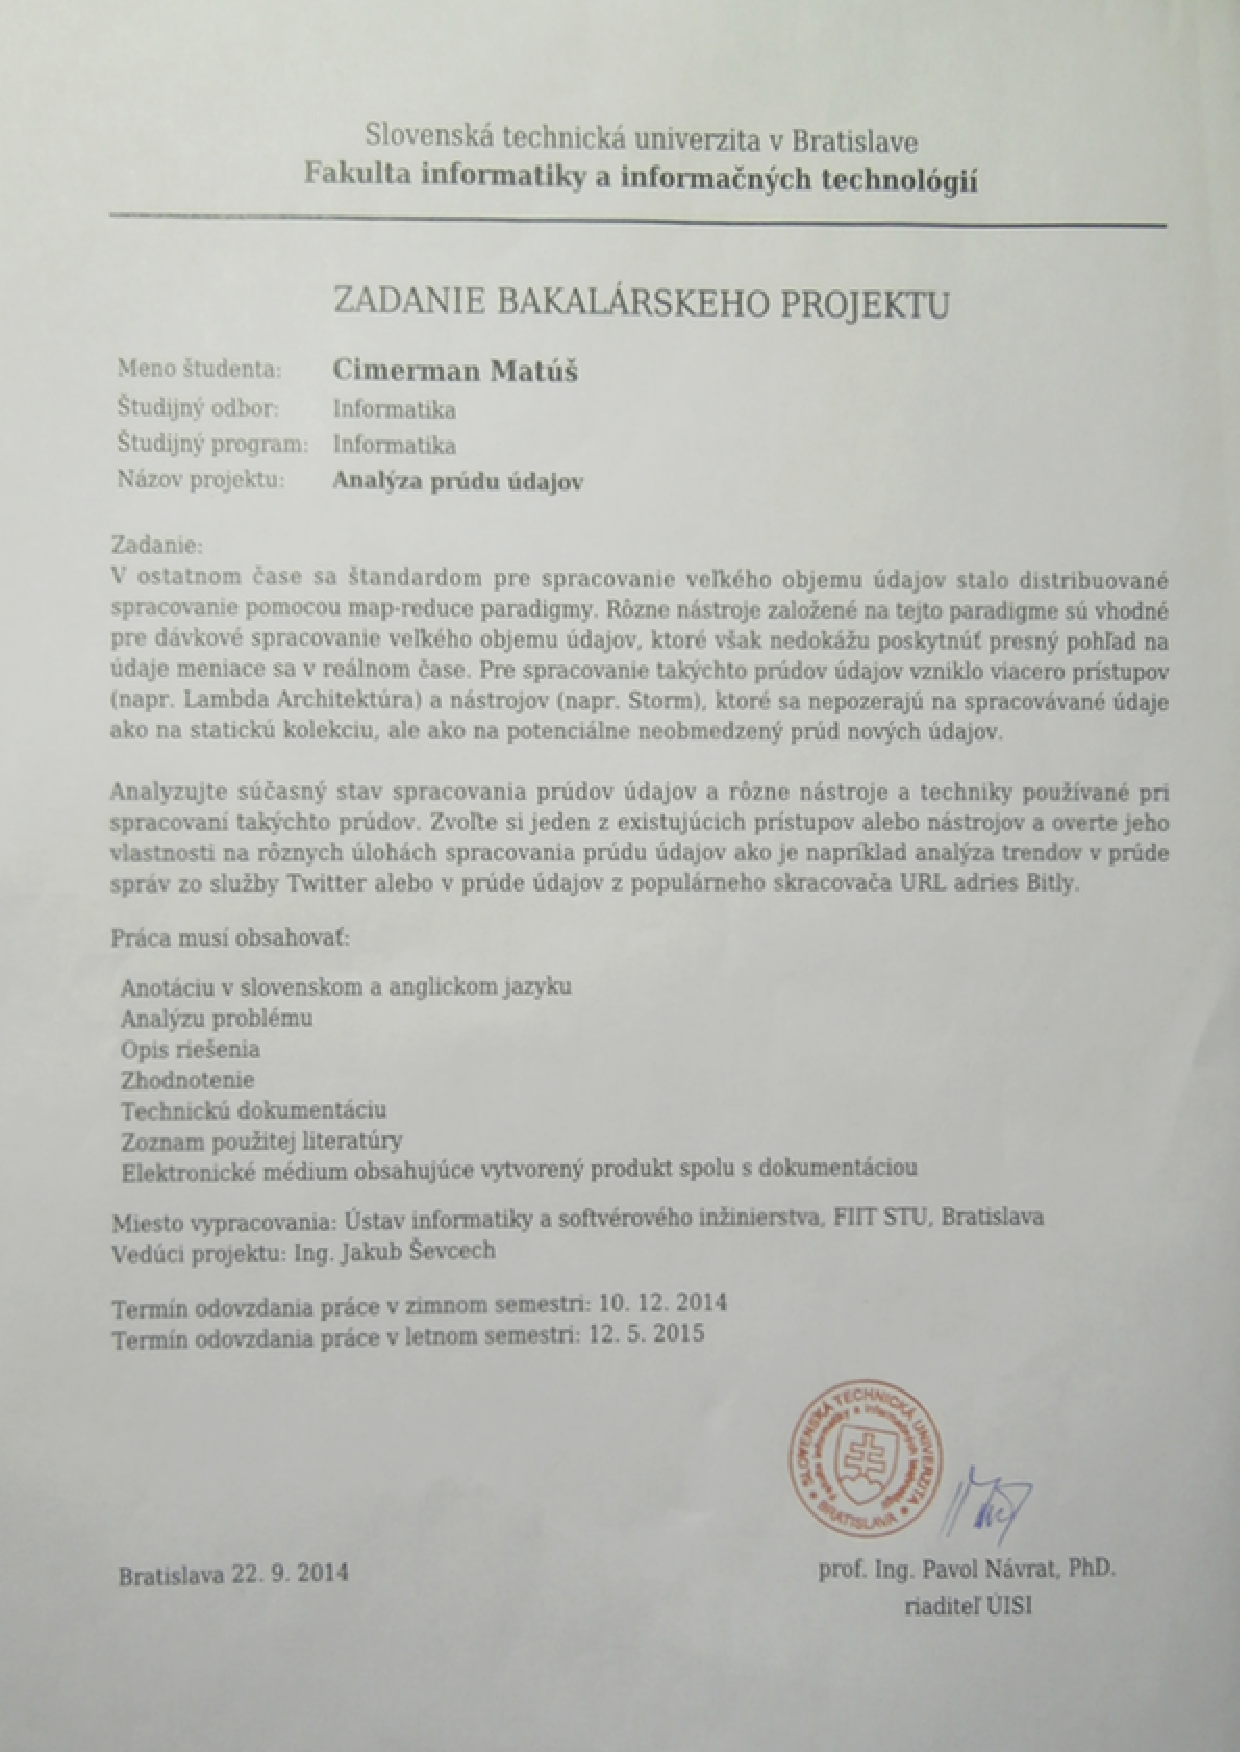
\includepdf[pages={1}]{ZADANIE.pdf}

%the abstract should include an english and a slovak version
%!TEX root = ./main.tex

% This file is part of the i10 thesis template developed and used by the
% Media Computing Group at RWTH Aachen University.
% The current version of this template can be obtained at
% <http://www.media.informatik.rwth-aachen.de/karrer.html>.

\loadgeometry{myAbstract}

\chapter*{Abstract\markboth{Abstract}{Abstract}}
\addcontentsline{toc}{chapter}{\protect\numberline{}Abstract}
\label{abstract}

%english version
Nowadays we can see Big Data processing and analysis in many domains. As a amounts of data growing, more people are focusing on this problem. The most affected domains are social media websites like Facebook or Twitter. A data from such a sources are streaming in huge amounts and changing in real-time, called data streams. We want to process and analyze data streams in real-time to provide users personalized and valuable outputs. The most common approach to handle data streams is map-reduce paradigm, e.g. batch data processing. Proposed methods are not meeting our requirement to process data streams in real-time. To achieve these requirements, we need use different approach called data stream processing which is built on Lambda Architecture.\\
Processing and analysis of big data streams is a complex task, because we need to provide low-latency, scalable and fault-tolerant solution. In our project, we analyze existing solutions and frameworks to analyze data streams. We provide verification of its characteristics in different kind of tasks. Accordingly to this, we propose a application for processing and analyzing big data streams (e.g. Twitter data stream), which allows users to get valuable outputs changing in real-time.\\
\todo{upravit anglicku podla slovenskej. V slovenskej su male upravy...- az po revizii slovenskej}
\emptydoublepage
\chapter*{Abstrakt\markboth{Abstrakt}{Abstrakt}}
\addcontentsline{toc}{chapter}{\protect\numberline{}Abstrakt}
\label{abstrakt
%slovak version
Dnes sa stretávame so spracovaním a anlýzou veľkého objemu dát v mnohých oblastiach. S narastajúcim objemom dát rastie aj záujem o tento problem spracovania veľkého objemu dát. Toto najviac postihuje oblasť sociálnych medií, napríklad Facebook, či Twitter. Dáta z takýchto zdrojov prúdia v obrovkých množstvách, pričom dáta sa v čase menia, takéto prúdiace dáta nazývame jednoducho prúd dát. Prúdy dát chceme spracovať a analyzovat v reálnom čase, aby sme mohli ponúknuť používateľom personalizovaný a hodnotný výstup. Najčastejší prístup spracovania prúdu dát je map-reduce paradigma, napríklad dávkové spracovanie. Táto metóda, ale nespĺňa naše požiadavky na spracovanie dát v reálnom čase. Na dosiahnutie našej požiadavky potrebujeme iný prístup, ktorý nazývame spracovanie prúdu dát. Metóda takéhoto prístupu je postavená na Lambda architektúre.
Spracovanie a analýza veľkých prúdov dát je komplexný problém, pretože prúd musí byť spracovaný s nízkou odozvou, riešenie musí byť odolné proti chybám a  škálovateľné. V našej práci budeme analyzovať existujúce riešenia and rámce na analýzu prúdu dát. Poskytujeme overenie charakteristík týchto riešení v roznych problémoch, ktoré si vyžadujú spracovanie prúdu dát v reálnom čase. Na základe tohto poskytujeme aplikáciu, ktorá spracuje a analyzuje veľký prúd dát (napríklad prúd dát Twittru), ktorá umožní používateľom získať hodnotný výstup, ktorý sa mení v reálnom čase.\\
\todo{zrevidovat slovensku verziu}
%Slovenska verzia.
\emptydoublepage
\loadgeometry{myText}

\emptydoublepage

%acknowledgements
\loadgeometry{myAbstract}

\chapter*{Poďakovanie\markboth{Poďakovanie}{Poďakovanie}}
%\addcontentsline{toc}{chapter}{\protect\numberline{}Poďakovanie}

\vfill
Na prvom mieste sa chcem poďakovať vedúcemu mojej bakalárskej práce, inžinierovi Jakubovi Ševcechovi za všetky jeho rady, odovzdané skúsenosti a výborne vedenie pri tvorení práce.\\
Ďalej sa chcem poďakovať všetkým výskumníkom zo skupiny PeWe za hodnotné diskusie počas celého semestra a tiež spätnú väzbu k mojej práci.\\
V neposlednom rade sa chcem poďakovať celej mojej rodine a priateľom.

\begin{flushright}
Matúš Cimerman
\end{flushright}


\loadgeometry{myText}


\emptydoublepage

%conventions applied in the thesis
%%!TEX root = ./main.tex
%
% This file is part of the i10 thesis template developed and used by the
% Media Computing Group at RWTH Aachen University.
% The current version of this template can be obtained at
% <http://www.media.informatik.rwth-aachen.de/karrer.html>.

\chapter*{Conventions\markboth{Conventions}{Conventions}}
\addcontentsline{toc}{chapter}{\protect\numberline{}Conventions}

Throughout this thesis we use the following conventions.



\bigskip

\emph{Text conventions}

Definitions of technical terms or short excursus are set off in coloured boxes.

\myDefBox{Excursus}
{Excursus are detailed discussions of a particular point in a book, usually in an appendix, or digressions in a written text.}

\medskip

Source code and implementation symbols are written in typewriter-style text.

\texttt{myClass}

\medskip

The whole thesis is written in Canadian English.

\medskip

Download links are set off in coloured boxes.

\myDownloadURL{File: myFile}{file_number.file}{file\myUnderscore number.file}

%\pagebreak

%\emph{Formula conventions}




%\emptydoublepage

\renewcommand{\contentsname}{Obsah}
\singlespacing
\tableofcontents

\emptydoublepage
\onehalfspacing
%\doublespacing
%
%\listoffigures
%\emptydoublepage
%
%\listoftables
%\emptydoublepage


%--------------------------------------------------------------
% hlavny obsah
%--------------------------------------------------------------
\mainmatter

%!TEX root = ./main.tex
%
% This file is part of the i10 thesis template developed and used by the
% Media Computing Group at RWTH Aachen University.
% The current version of this template can be obtained at
% <http://www.media.informatik.rwth-aachen.de/karrer.html>.

\chapter{Úvod}
%\label{introduction}
\todo{napisat uvod} 


\emptydoublepage
\chapter{Modely spracovania údajov}
\label{Data streams overview and processing methods}
V tejto kapitole sa venujeme metódam, či prístupom k spracovaniu veľkého objemu údajov (angl. Big Data). Dávkové spracovanie je jednou z najčastejšie používaných metód spracovania big data, ale jej použitie zlyhýva v aplikáciach, pri ktorých môže byť čas odozvy kritický. Môžu to byť napríklad aplikácia, ktorá spracuje údaje zo senzorov lietadla alebo aplikácia na analýzu trendov na sociálnej sieti. Z tohto dôvodu v tejto kapitole porovnávame dva prístupy spracovania big data, \textit{dávkové spracovanie} (angl. batch processing) a \textit{prúdové spracovanie} (angl. stream processing), pričom druhá metóda hovorí, ako to vyplýva z názvu, o spracovaní prúdu dát.
\par
Najskôr je potrebné čo najpresnejšie definovať, čo je to prúd údajov. Prúd údajov môže naberať iný význam v závilosti na zdroji týchto údajov. Vo všeobecnosti, je ale prúd dát, potenciálne nekonečný a nijak ohraničený tok dát v pohybe. Takýto prúd má tri význačné vlastnosti, veľký \textit{objem} (angl. volume), vysokú \textit{premenlivosť} (angl. velocity) a \textit{pestrosť} (angl. variety) prúdiacich správ za jednotku času\citep{kaisler2013big}. Pre priblíženie, objem sa pohybuje rádovo v stovkách tisícov správ za sekundu. Ako príklad môžme uviesť aktivitu na sociálnej sieti Twitter, ktorá presahuje 50 milionóv nových správ (tweetov) za jeden deň\citep{mathioudakis2010twittermonitor}.
\par
Najčastejšie zdroje takýchto dát, ktoré vyžadujú prúdové spracovanie dát v reálnom čase pre dosiahnutie hodnotných výstupov:
\begin{itemize}
    \item \textit{sociálne média} ako napríklad Twitter, či Facebook produkujú masívny objem dát v reálnom čase, ktoré strácajú svoju informačnú hodnotu veľmi rýchlo.
    \item \textit{údaje z logovacích súborov}, webové servery, databázy a rozne iné zariadenia produkujú súbory, do ktorých sú ukladané logy.
    \item \textit{sieťové zariadenia alebo prvky} kontinuálne generujú hodnotné dáta v obrovských objemoch, tiež v závislosti na veľkosti siete.
    \item \textit{senzory a snímače}, ktoré môžu merať fyzikálne veličiny.
\end{itemize} 
Takéto prúdy má zmysel spracovať v reálnom čase, aby sme dosiahli hodnotné výstupy. Spracovanie v reálnom čase sa môže opäť meniť v kontexte problému. V našom prípade to bude najčastejšie znamenať, že správnosť výsledku nebude závislá iba na jeho správnosti, ale aj na čase za aký bude poskytnutý \citep{stankovic1999misconceptions}. \\

Pre získanie hodnotného výstupu na základe dopytu používateľa je nutné vykonať operáciu nad všetkými dostupnými dátami\citep[s. 8-10]{marz2013big}.
\begin{center}
\textit{dopyt = fn(všetky dáta, ktoré sú k dispozícií)}
\end{center}

% Vlastnosti systemu na spracovanie big data
%\paragraph{Žiadúce vlastnosti architektúry na spracovanie veľkého objemu dát}
Pri navrhovaní architektúry softvérového systému, ktorá ma za úlohu spracovať veľký objem dát je nevyhnutné aby spĺňala aspoň tieto nasledujúce vlastnosti:
\begin{enumerate}
    \item \textit{robustná a odolná voči chybám}, architektúra je robustná, ak bez chyby odolá nečakaným stavom, ako napríklad výpadok elektrickej energie. Je odolná voči chybám, ak chybné dáta alebo strata dát nemá za následok poškodený výstup.
    \item \textit{nízka odozva}, aplikácie postavené na tejto architektúre sú schopné poskytnúť odozvu v požadovanom čase. Typicky rádovo desiatky, maximálne stovky milisekúnd.
    \item \textit{horizontálne škálovateľná}, ak je možné zvýšiť výkon celej architektúry pridaním fyzického uzla bez dopadu na funkcionalitu.
    \item \textit{všeobecná}, architektúru je možné použiť na rôzne aplikácie.
    \item \textit{rozšíriteľná}, do fungujúcej architektúry je možné pridávať novú funkcionalitu za prijateľnej námahy.
\end{enumerate}




%\section{Tradičné prístupy k spracovaniu dát}
%\textbf{TODO: spracovanie prudu tradicnym pristupom pomocou relacnych databaz - najprv ulozit data a potom snimi pracovat }


% DAVKOVE SPRACOVANIE %
\section{Dávkové spracovanie veľkého objemu dát}
Dávkové spracovanie veľkého objemu dát funguje na príncipe, ako napovedá názov, spracovania dát v dávkach. Nespracujú sa všetky dáta naraz, alebo postupne ako vznikajú, ale v istých dávkach. Tieto dávky môžu byť rozne veľké. Môžu byť ohraničené časovo alebo veľkosťou. Najčastejší prístup je vytvárať dávky na spracovanie po nejakých časových intervaloch, napríklad každých sedem hodín. Znamená to, že po dobu sedem hodín niekam akumulujeme nové dáta. Po uplynutí tohto času je nad týmito dátami a všetkými, ktoré boli doteraz zaznamenané, vykonaná nejaká operácia (napríklad priemer čísel) a jej výsledok je uložený vo forme \textit{pohľadu}. \\

\myFrameBigFigure[]{davkove.eps}{Obrázok zobrazuje dávkové spracovanie dát, pričom na pravej strane sú vytvárané rôzne pohľady.}{Dávkové sprac. dát}
S takýmto prístupom bude len veľmi ťažké dosiahnut nízku odozvu na dopyt používateľa. Nakoľko minimálne v jednom momente bude \textit{pohľad} sedem hodín neaktuálny. Tomuto by sa teoreticky dalo zabrániť rapídnym znížením časového intervalu.
\par
Pri tomto prístupe sú všetky dáta ukladané do databázy, tak ako prišli. Nie sú vôbec modifikované, takže sa pracuje s čistými dátami. Súbor dát, ktorý uchovávame môže byť preto veľmi objemný, rádovo terabajty. To znamená, že každé spracovanie dávky je časovo a výpočtovo náročná operácia a môže niekedy trvať aj celé hodiny. 
\par 
Nami poskytnuté teoretické riešenie ako sa vyhnúť vysokej odozve znížením časového intervalu, po ktorom je vykonané dávkové spracovanie, by nebolo riešením.
To čo sa môže zdať ako nevýhoda, je zároveň aj výhoda, pretože ukladaním všetkých dát dosahujeme odolnosť voči chybám (aj spôsobným človekom) a pri vytváraní pohľadu zohľadňujeme údaje z minulosti. 
\par
Dávkové spracovanie dát nám poskytuje distribuované a spoľahlivé (tj. odolné voči chybám) riešenie. Tento prístup tiež poskytuje škálovateľnosť, je dostatočne všeobecný a rozšíriteľný. Avšak neposkytuje nízku odovzu. Nasledujúci zoznam hovorí o najdôležitejších vlastnostiach dávkového spracovania:
\begin{enumerate}
    \item \textit{neohraničené počítanie}, znamená že máme teoreticky neobmedzenú výpočtovú silu a neobmedzený čas výpočtu. Teoreticky môžeme vykonať dávkové spracovanie nad akýmkoľvek dátovým súborom.
    \item \textit{ukladanie normalizovaných dát}, neexistuje potreba dáta denormalizovať, pretože pohľady sú generované často.
    \item \textit{architektúra je horizontálne škálovateľná}.
%    \item \textit{vykonáva len zápis}, žiadne dáta sa nie sú vymazané.
    \item \textit{dáta sú konzistentné}, za predpokladu, že vstupné dáta sú korektné.
\end{enumerate}

\subsection{Metódy dávkového spracovania}
\paragraph{MapReduce} je programovací model a príslušná implementácia na spracovanie a generovanie masívnych údajových korpusov \citep{Dean2008}. Tento model bol vymyslený kvôli výpočtovej zložitosti a problému distribuovať a paralelizovať výpočet. Je založený na primitívach prezentovaných v programovacom jazyku Lisp, \textit{mapovanie} a \textit{filtrovanie}. Výpočet je vykonávaný za použitia len týchto dvoch funkcií. Funkcia \textit{mapovanie} má ako vstupný argument dvojicu \textit{kľúč/hodnota} s kľúčom \textit{K}, nad ktorou spraví používateľom definovanú operáciu, a vytvorí dočasnú dvojicu s kľúčom \textit{K}. Túto hodnotu s kľúčom \textit{K} ďalej konzumuje funkcia \textit{filtrovanie}, ktorá najčastejšie spojí hodnoty do jednej (napríklad operácia sčítania). Ako jednoduchý príklad uvádzame problém spočítania výskytov slova vo veľkej kolekcii dokumentov \citep{Dean2008}:

\paragraph{Dátové kocky} (angl. Data cubes)
Dátová kocka, tiež známa pod pojmom OLAP\footnote{Online Analytical Processing} kocka, je dátová štruktúra, ktorá umožňuje rýchlu analýzu dát. Hlavná motivácia prečo vytvárať dátove kocky je materializácia všeobecných údajov. Takáto kocka má dve hlavné atribúty, \textit{dimenzia} a \textit{hodnota}. Pričom dimenzie predstavujú nezávislé hodnoty, napríklad vek a hodnota je závislá, pretože bude viazaná k veku v konkrétnom zázname. Viac rozmerný priestor je vymedzený dimenziami kocky. Nad dátovými kockami poznáme niekoľko základných operácií, \textit{krájanie} (angl. slicing), \textit{delenie} (angl. dicing), \textit{pivotovanie} (angl. pivoting), \textit{zrolovanie} (angl. roll up), \textit{drill-down}\citep{franekimporty}. 

\paragraph{Hviezdicová schéma} (angl. Star schema)
Hviezdicová schéma sa používa na modelovanie viac dimenzionálnych dát a vychádza priamo z princípov relačných databáz. Pričom priamo v tabuľke je uložených len niekoľko základných faktov a kľúčov. Tieto kĺúče ďalej odkazujú na ďalšie tabuľky, ktoré môžu odkazovať na ďalšie tabuľky\citep{chaudhuri1997overview}. Dopytovanie sa do takéjto schémy je pomerne efektívne, nakoľko nie je vždy potrebné dotazovanie vo všetkých dimenziách.

\paragraph{Dátové sklady} (Datawarehouse)
Pojem dátový sklad definoval v roku 1990 Bill Inmon. Dátovy sklad je subjektovo orientovaná, integrovaná, stála a časovo rozdielna kolekcia dát podporujúca rozhodujúce procesy\citep{chaudhuri1997overview}. Dátové sklady nám poskytujú zovšeobecnené a ustálené dáta vo viacerých dimenziách. Dátové sklady nám tiež poskytujú prostriedky ako napríklad OLAP, ktorý bol vyšie spomenutý v súvislosti s dátovými kockami. Dátove sklady sú typicky udržiavané mimo hlavnej databázy, resp. úložiska dát. 





% PRUDOVE SPRACOVANIE %
\section{Prúdové spracovanie dát}
Správne fungovanie niektorých aplikácií je priamo závislé na takmer okamžitom výsledku z nekonečného spojitého prúdu dát. Keďže prúd je nekonečný, nové dáta prichádzajú kontinuálne a teda aj výsledky a zmeny z nich vyplývajúce. Dáta musia byť spracované tak ako prichádzajú. Spracovanie takýchto nekonečných prúdov dát aplikovaním tradičných metód môže byť problém, keďže výpočtové prostriedky sú limitované \citep{babcock2002models}. Množstvo predtým (rádovo sekundy) vygenerovaných dát je zvyčajne veľké a preto sú často po spracovaní zahadzované, ale môžu byť uložené na disku. V prípade keby sme aj chceli pristupovať k dátam z minulosti (môže byť užitočné pri detekcii trendov) bolo by to výpočtovo náročné, pretože dopyt sa musí vykonať nad všetkými doteraz uloženými dátami pre získanie jedného výstupu\citep{silvestri2006distributed}. Na tkéto uloženie sa najčastejšie používajú NoSQL databázy, pretože tradičné extrahuj-transformuj-načítaj (ETL)\footnote{extract-transformation-load} relačné databázy sú priveľmi štrukturované a pomalé \citep{liu2014survey}. Preto sa budeme zaoberať v tejto kapitole iba nástrojmi, ktoré adresujú spracovanie v takmer-reálnom čase.
\par
Pri prúdovom spracovaní sa stretávame s niekoľkými špecifikami:


\paragraph{Prúd dát}

\paragraph{Problémy}



































\emptydoublepage
\chapter{Existujúce riešenia modelov spracovania údajov}
\label{Existing solutions of data stream analysis} 
V tejto kapitole bližšie rozoberieme existujúce riešenia, ktoré sme analyzovali. Zamerali sme sa najmä na riešenia, ktoré nie sú proprietárne. Existujúce riešenia je možné rozdeliť do dvoch skupín a to, dávkové a prúdove spracovanie údajov. 

%  ================= Davkove spracovanie  ================= %
\section{Dávkové spracovanie}
Analyzovali sme riešenia dávkového spracovania veľkého objemu údajov (angl. Big Data). Nástroje aplikujúce princípy dávkového spracovania pracujú väčšinou so statickou kolekciou dát. Tieto nástroje poskytujú možnosti spracovania a analýzy masívnych objemov dát, niektoré nástroje dovoľujú spracovať chybné a neúplné údaje. Spracovanie nie je v reálnom čase, výpočet je vykonávaný periodicky a trvá v závislosti na objeme korpusu rádovo sekundy, minúty, či hodiny a viac.

%  ================= HADOOP  ================= %
\subsection{Hadoop} 
\label{hadoop-exists}
Apache Hadoop\footnote{Apache Hadoop: https://hadoop.apache.org/} je populárna open source 
%\footnote{Open-source je akákoľvek informácia dostupná širokej verejnosti, za predpokladu, že môže byť bez postihnutia šírená ďalej v pôvodnom alebo upravenom stave. To do akej mieri je možné open source upravovať často definuje licencia. Tento pojem vznikol z pri definovaní open source softvéru, dnes sa však už môže viazať na takmer čokoľvek.}
implementácia MapReduce programovacieho modelu. Hadoop pozostáva z dvoch základných komponentov: Distribuovaný Súborový Systém Hadoop \textit{HDFS} (angl. Hadoop Distributed File System) a \textit{MapReduce} programovacieho rámca \citep{liu2014survey}. Obidva komponenty sú postavené na architektúre \textit{otrokár-otrok} (angl. master-slave). Hadoop program, alebo klient, odosiela \textit{prácu} (angl. job) cez \textit{stopovač práce} (angl. jobtracker), ktorý beží na serveri, do MapReduce rámca. Stopovač práce priraďuje úlohy \textit{stopovačovi úloh} (angl. tasktracker), ktorý beží na mnohých slave uzloch. Stopovač úloh posiela pravidelné \textit{správy}\footnote{Často nazývané údery srdca (angl. heartbeats) sú správy, ktoré informujú master uzol a stave slave uzlov a úloh.} informujúce stopovač práce o statuse jeho úloh, napríklad \textit{čakajúca}, \textit{činná}, \textit{zaneprázdnená}, atď. Ak vykonávaná úlohá zlyhá, vyprší časový limit alebo uzol, na ktorom je úloha vykonávaná, bude nejakých príčin bude vypnutý, stopovač úloh môže automaticky preplánovať úlohu na iné živé uzly v klastri. 
  \\[5pt]
 Ďalší komponent Hadoop HDFS (obr. 3.1) pozostáva z jedného menného uzla (angl. namenode) a viacerých \textit{dátových uzlov} (angl. datanode) Namenode udržuje metadáta dát udržovaných v dátových uzloch. Ak chce klientská aplikácia zapisovať alebo čítať z HDFS musí najprv komunikovať s namenode odkiaľ získa pozíciu dátového bloku, z ktorého môže čítať alebo zapisovať. Metadáta sú načítané do hlavnej pamäti pri štarte Hadoop-u. Dátové uzly, podobne ako stopovač úloh, aktualizujú stav menného uzla. 
 \myFrameBigFigure[H]{images/IMG_existujuce-hadoop}{Hadoop distribuovaný súborový systém (HDFS) s replikáciou dát a klientom, ktorý číta niektoré dátové uzly.}{existujuce-hadoop}
 \\[1pt]
 Hadoop MapReduce rámec je navrhnutý s cieľom dosiahnuť horizontálnu škálovateľnosť a odolnosť voči chybám, ale nie je optimalizovaný pre rýchle vstupno/výstupné operácie. Odolnosť voči chybám je zabezpečená správnou implementáciou modelu MapReduce, o čom sme viac hovorili v podkapitole \ref{metody-davkove}. Problém MapReduce rámca je chýbajúce plánovanie vykonávania kvôli optimalizácií výpočtu a komunikácie v strapci. Aj v prípade efektívneho plánovania úloh a komunikácie naprieč strapcom je stále Hadoop systémom dávkového spracovania údajov kvôli jeho povahe spracovania dát.
 
 %  ================= EasyBatch ================= %
% \newpage
\subsection{EasyBatch}
EasyBatch\footnote{EasyBatch: http://www.easybatch.org/} je Java programovací rámec zameraný na zjednodušenie dávkového spracovania dát. Hlavný cieľ je zjednodušiť často používané operácie nad dátami ako napríklad čítanie, filtrovanie, parsovanie a validácia vstupných dát. EasyBatch môže bežať samostane alebo spustený na aplikačnom serveri. Rámec má niekoľko hlavných vlastností: \textit{jednoduchosť} (pozn.: jadro nemá žiadne závislosti, a preto zaberá málo miesta na disku ~ 80kB), \textit{POJO\footnote{Plain old Java Object je nijak obmedzený obyčajný Java objekt}} orientovaný vývoj, \textit{deklaratívna validácia dát}, \textit{generovanie reportov}, \textit{monitoring} dávkového spracovania, \textit{paralelné spracovanie}. Tento rámec je síce vytvorený na dávkové spracovanie dát, ale nie je horizontálne škálovateľný, aspoň nie v jeho podstate bez pridania externých programov a ďalšieho úsilia, narozdiel od Hadoop-u.

 %  ================= misco ================= %
\subsection{Misco}
Distribuovaný programovací rámec Misco\footnote{Misco: http://alumni.cs.ucr.edu/~jdou/misco/} \citep{dou2010misco} je určený pre mobilné zariadenia. Rámec je implementovaný v programovacom jazyku Python vďaka čomu by ho malo byť jednoduché portovať na všetky platformy, ktoré podporujú tento jazyk a jeho knižnice na sieťovú komunikáciu. Je založený na MapReduce modeli, je potrebné programovať len funkcie Map a Reduce, o ostatné sa postará rámec, t. j. distribúcia kódu a dát, paralelné spracovanie, plánovanie a zlyhania uzlov. Misco systém pozostáva z hlavného serveru a viacerých klientských uzlov, na ktorých prebieha výpočet. Hlavný server zodpovedá za sledovanie stavu klientských uzlov, distribúciu dát, plánovanie a priraďovanie úloh. Klientské uzly sú, naopak, zodpovedné za to, aby si dopytovali úlohy na spracovanie od serveru vykonaním operácie nad dátami a vratením výsledku serveru. 

 %  ================= Disco ================= %
\subsection{Disco}
Disco\footnote{Disco: http://discoproject.org/} je implementácia MapReduce modelu pre distribuované dávkové spracovanie. Disco podporuje paralelné spracovanie veľkých dátových korpusov. Jadro je napísané vo funkcionálnom jazyku Erlang, ktorý bol vytvorený na budovanie robustných distribuovaných aplikácií odolných voči chybám. Disco je postavený na otrokár-otrok (angl. master-slave) architektúre. \textit{Otrokár} (master) prijíma \textit{práce} (angl. jobs), ktoré distribuuje na vykonanie naprieč klastrom uzlov. \textit{Klienti} odosielajú \textit{práce} do hlavného uzla (otrokár). Podradené uzly (otrok) hlavnému uzlu sú ním tiež riadené a monitorované. V klastri Disco môže existovať viac hlavných uzlov.

%%%%%%%%%%%%%% PRUDOVE %%%%%%%%%%%%
%\newpage
\section{Prúdové spracovanie}
Prúdové spracovanie v dnešnej dobe získava stále vyššiu pozornosť a záujem. Keďže sa v našej práci venujeme najmä prúdovému spracovaniu, v tejto časti analyzujeme viacero nástrojov vytvorených na spracovanie prúdu údajov.

 %  ================= S4 ================= %
\subsection{S4}
Skratka S4 znamená \textit{Jednoduchý Škálovateľný Prúdový Systém} (angl. \underline{S}imple \underline{S}calable \underline{S}treaming \underline{S}ystem, S4). Tento systém je založený sčasti na modeli MapReduce. S4 je všeobecná, distribuovaná a škálovateľná platforma, ktorá je \textit{čiastočne} odolná voči chybám. Napríklad, ak spracujúci uzol v topológií zlyhá kvôli chybe, spracovanie je automaticky presunuté na iný uzol, ale stav pôvodného uzla je stratený, a nemôže byť obnovený \citep{neumeyer2010s4}.
 \\[5pt]
Tento systém nepoužíva zdieľanú pamäť a je založený na modeli Hráčov (angl. Actor model) v kombinácií so spomenutým modelom MapReduce. S4 má decentralizovanú symetrickú architektúru, v ktorej sú všetky uzly na rovnakej úrovni (rozdiel oproti otrokár-otrok architektúre). Tieto uzly sú nazývané \textit{spracujúce elementy} (angl. processing elements, ďalej len PE). S4 si vymieňa informácie medzi PEs vo forme dátových udalostí, čo je aj jediná možnosť interakcie a výmeny informácií medzi PEs. Klaster (angl. cluster) S4 pozostáva z PEs na spracovanie týchto udalostí. Vzhľadom na to, že dáta prúdia medzi PEs a výpočet beží len v hlavnej pamäti PE, nie je potrebné ukladanie na disk. Z toho vyplýva už spomenutá, čiastočná odolnosť voči chybám. 
 \\[5pt]
Pretože v systéme neexistuje žiadny hlavný uzol (master), ktorý by sa staral o uzly, kde prebieha výpočet (slave), ale sú všetky uzly na rovnakej úrovni je potrebné zabezpečiť manažment klastra uzlov. Toto je mnohokrát vyriešené platformou ZooKeeper\footnote{ZooKeeper: https://zookeeper.apache.org/}. ZooKeeper je centralizovaná platforma na manažment distribuovaných aplikácií.

 %  ================= Spark ================= %
\subsection{Spark}
Spark \citep{liu2014survey} je klastrový výpočtový systém. Kombinuje spracovanie uložených dát v dávkovom móde so spracovaním prúdu údajov v reálnom čase. Dávková čast Spark-u je postavená na Hadoop HDFS opísaná podrobnejšie v kapitole \ref{hadoop-exists} Hadoop.
Cieľom Spark-u je poskytnúť rýchlu výpočtovú platformu pre analýzu dát. Spark poskytuje všeobecný model výkonávania ľubovolných dopytov, ktoré sú výkonávané v hlavnej pamäti (pokiaľ ide o prúdové spracovanie). Tento model je nazvaný \textit{Pružný distribuovaný dataset}, skr. RDD (angl. Resilient Distributed Dataset), čo je dátova abstrakcia distribuovanej pamäti. Keďže výpočet beží v hlavnej pamäti (pri prúdovom spracovaní), nie je potrebné vykonávať zápisy na disk, vďaka čomu môže byť dosiahnuté spracovanie v reálnom čase. Výpočet prebieha vo veľkom klastri uzlov s dosiahnutím odolnosti voči chybám za použitia RDD. RDD  sídli v hlavnej pamäti, ale môže byť periodicky ukladaný na disk. Vďaka distribuovanej povahe RDD môže byť stratená časť RDD obnovená z pamäti iného uzla. Samotné prúdové spracovanie nie je vykonávané správa po správe (angl. message by message), ale v mikro dávkach, ktoré môžu byť automaticky paralelne distrubované v strapci.

 %  ================= IBM InfoSphere streams ================= %
 %doplnit infosphere streams, AK vyjde cas
%\subsection{IBM InfoSphere Streams}

 %  ================= Samza ================= %
\subsection{Apache Samza}
Apache Samza \citep{kamburugamuvesurvey} je programovací rámec pre prúdové spracovanie vyvinutý firmou LinkedIn\footnote{LinkedIn: https://www.linkedin.com/}. Prúd správ je neohraničená nemenná kolekcia správ rovnakého typu. Prúd môže byť čítaný viacerými konzumetami v systéme, a správy môžu byť pridávané alebo odstraňované z prúdu. Prúdy sú vždy udržiavané na úrovni \textit{dohadzovačov} (angl. broker). Práca (angl. job) je logická kolekcia výpočtových jednotiek alebo uzlov, ktoré spracujú prúd a vytvárajú výstupný prúd dát. Táto kolekcia vytvára sieťovú topológiu, ktorá spracuje správy. Prúdy su rozdeľované do pod prúdov, ktoré sú distribuované a spracované paralelne. Úloha predstavuje PE (processing element) v Samza rámci. Jedna úloha môže emitovať jeden výstupný prúd, ale na vstupe môže byť viacero vstupných prúdov. 
\\[5pt]
Distribuované plánovanie a prideľovanie prostriedkov sa spolieha na Apache Yarn\footnote{Apache Hadoop NextGen MapReduce (YARN): http://hadoop.apache.org/docs/current/hadoop-yarn/hadoop-yarn-site/YARN.html}, o distribuované posielanie údajov sa stará Apache Kafka\footnote{Apache Kafka je publish-subscribe distribuovaný systém správ: http://kafka.apache.org/}. Architektúra Samza je zobrazená na obrázku 3.2.
Klaster Samza uzlov je manažovaný Yarn-om. Systém je optimalizovaný pre spracovanie veľkého objemu správ a poskytuje možnosť ukladať správy na disk pre dávkové spracovanie. Samza využíva rozdeľovanie správ podľa tém (topic) systému Kafka na dosiahnutie distribuovaného rozdelenia prúdu v strapci. Uzol v Samza strapci môže konzumovať správy z Kafka komunikačného systému správ, ale tiež produkovať nový prúd správ do Kafka sprostredkovateľov. 
\myFrameBigFigure[]{images/IMG_existujuce-samza}{Samza architektúra postavená na Apache Yarn a Apache Kafka, zdroj: \citep{kamburugamuvesurvey}.}{existujuce-samza}
\\[5pt]
Samza poskytuje garanciu a odolnosť voči chybám a doručenia správ \textit{aspoň raz} (angl. at least once). Ak nejaký uzol zlyhá, nastane preplánovanie úlohy do iného uzla, ktorý prevezme čítanie správ danej témy od sprostredkovateľa (sprostedkovateľ si udržuje zadefinovaný časový úsek správ). Keďže táto odolnosť voči chybám je dosiahnutá prostredníctvom Kafka sprostredkovateľov, ak nastane výpadok alebo chyba v sprostredkovateľoch, Samza stratí správy, ktoré nemôžu byť obnovené. Replikáciou súborového systému sprostredkovateľov je možné sa tomuto vyhnúť.

 %  ================= STORM ================= %
\subsection{Apache Storm}
\label{existujuce-storm-subkap}
Apache Strom\footnote{Apache Storm: https://storm.apache.org/} \citep{liu2014survey, kamburugamuvesurvey} je programovací rámec vytvorený na spracovanie prúdu dát. Je to open-source riešenie, ktoré poskytuje spracovanie prúdu dát s nízkou odozvou. Storm je navrhnutý aby poskytol odolnosť voči chybám (garancia doručenia správ), robustnosť a škálovateľnosť. 
\\[5pt]
Architektúra Storm-u zobrazená na obrázku 3.3 pozostáva z viacerých častí, koordinátora uzlov klastra ZooKeeper, manažérov stavov Nimbus\footnote{Nimbus: http://www.nimbusproject.org/} a spracovávajúcich uzlov Supervisor\footnote{Supervisor: http://supervisord.org/}. Nimbus je hlavný server, kde sa nahráva klientský kód na vykonanie. Tento kód je Nimbus-om distribuovaný v rámci \textit{pracovníkov} (workers) v strapci. Nimbus si tiež udržuje status všetkých pracovníkov, takže sa stará o prípadné reštarty alebo presun \textit{úloh} (task) v prípade zlyhania niektorého pracovníka. Množina pracovníkov v klastri Storm-u beží na pozadí ako démon Supervisor-a. ZooKeeper sa stará o koordináciu medzi uzlami Supervisor-a a hlavného servera Nimbus. Tok správ v systéme je zabezpečený komunikačným systémom správ ZeroMQ\footnote{ZeroMQ: http://zeromq.org/}.
\myFrameBigFigure[]{images/IMG_existujuce-storm}{Zjednodušná architektúra Storm-u a jej komponenty, zdroj: https://storm.apache.org/documentation/Tutorial.html}{existujuce-storm} 
\\[5pt]
Storm nie je prispôsobený žiadnemu konkrétnemu programovaciemu modelu (napríklad MapReduce model). Programovací model Storm-u postkytuje distribuované rozdelenie prúdu medzi uzly. Tento model pozostáva zo \textit{skrutiek} (angl. bolt) a \textit{prameňov} (angl. spout), \textit{topológií} a \textit{prúdov}. Skrutky a pramene sú logicky spojené v orientovanom acyklickom grafe (skr. DAG, angl. directed acyclic graph). Vytvárajú tak určitú sieť uzlov nazývanú topológia. Používateľ odosiela vytvorené topológie hlavnému serveru klastra Storm, ktoré sa majú vykonať v klastri Storm. Abstrakcia nad prúdiacimi údajmi sa v skratke nazýva prúd, čo je neohraničená sekvencia n-tíc. Prúdy môžu byť definované používateľom (udalosti z Twittru) alebo systémové prúdy (hodinový signál). Skrutky konzumujú údaje a môžu ďalej emitovať nové prúdy po spracovaní n-tice na vstupe. Pramene len produkujú správy vo forme prúdu n-tíc. Topológia Storm-u väčšinou začína niekoľkými prameňmi a ďalej nasledujú len skrutky, ktoré spracujú prúd. Práca (job), ktorú poznáme z dávkových systémov, v Storm-e predstavuje Java objekt topológie, ktorý je odoslaný do hlavného servera Nimbus. Nimbus sa už postará o distribúciu a vykonanie topológie v rámci klastra. Na obrázku 3.4 je ukážka jednoduchej topológie postavenej na programovacom rámci Storm. 
\myFrameBigFigure[]{images/IMG_existujuce-storm-2}{Ukážka topológie Storm-u}{existujuce-storm-2} 
\\[5pt]
Kód skrutiek môže byť vykonávaný vo viacerých úlohách pracovníka paralelne. Skrutky navzájom prepojené sú tiež vykonávané paralelne. Takto logicky prepojené skrutky si medzi sebou posielajú správy. Tieto správy musia prísť vždy do správnej úlohy v správnom vlákne, preto Storm zavádza pravidlá pre smerovanie správ medzi boltami. Presnejšie ide o to, ako budú správy zoskupované naprieč hranou medzi dvoma uzlami v grafe topológie. Správy môžu byť napríklad \textit{rovnomerne miešané} (angl. shuffle) medzi úlohami, vtedy väčšinou nezáleží na tom, ktorá skrutka spracuje ktorú správu. Niekedy je potrebné aby len konkrétna úloha vždy spracovala všetky správy obsahujúce nejaký atribút, alebo je žiadané replikovať správy do všetkých úloh. O toto sa tiež stará Storm implementáciou niekoľkých možností zoskupovania správ (angl. grouping) naprieč medzi uzlami. 
\\[5pt]
Odolnosť voči chybám je v Storm-e zabezpečená tak, že si každý uzol grafu drží výstupnú frontu správ. Správy vo fronte zostávajú, pokiaľ nie sú potvrdené (angl. acknowledged). Uzol ktorý správu spracuje ju potvrdzuje, po úspešnom spracovaní. V prípade, ak nepríde potvrdenie na správu, ktorá bola emitovaná do nejakého definovaného času, uzol preposiela správu znova. Tento mechanizmus je ohraničený len hlavnou pamäťou uzla, keďže Storm beží v hlavnej pamäti a posktyuje garanciu doručenia \textit{aspoň raz}. 
\\[5pt]
Zlyhania uzlov monitoruje hlavný server Nimbus, ktorý sa tiež stará o ich riešnie. Uzly supervisor-a posielajú pravidelné správy o svojom stave hlavnému serveru (heartbeats). Zlyhanie uzla a chyba správy sú dve ortogonálne udalosti, chyba alebo zlyhanie správy môže nastať chybou v sieti alebo chybou v softvéri. Manipulácia chybných správ a chybých uzlov preto prebieha úplne nezávisle odlišným spôsobom nezávisle od seba. Tento prístup robí systém ešte viac robustným.

 %  ================= Zhodnotenie ================= %
\section{Zhodnotenie existujúcich riešení}
V súčasnosti existuje veľké množstvo nástrojov na spracovanie veľkých objemov údajov (angl. Big Data). Pre dávkové spracovanie Big Data sa dnes používa majoritne Hadoop, ostatné riešenia nie sú tak robustné a často používané ako práve Hadoop. Pre zjednodušenie práce s Hadoop existuje, naviac, mnoho rozšírení resp. úzko súvisiacich projektov (napr. Hive\footnote{Hive, dátové sklady poskytujúce sumarizáciu dát: http://hive.apache.org/}, HBase\footnote{HBase, podpora štruktúrovaných údajov pre veľké dátové súbory: http://hbase.apache.org/}, Mahout\footnote{Mahout, strojové učenia sa a dolovanie dát: http://mahout.apache.org/}, Apache Pig\footnote{Apache Pig, vysoko úrovňový jazyk pre paralelné počítanie: http://pig.apache.org/}). 
Z množstva rôznych dostupných nástrojov na prúdové spracovanie je očividné, že v poslednej dobe zvyšuje vysokú pozornosť práve prúdové spracovanie. Na analýzu všetkých týchto nástrojov v tejto práci nie je priestor. 
\\[5pt]
Všetky nástroje pre prúdové spracovanie sú postavené na istej obdobe otrokár-otrok (angl. master-slave) architektúry. Niektoré sú odolné voči chybám a garantujú doručenie každej správy minimálne jedenkrát. Každé analyzované riešenie bolo distribuované a škálovateľné, čo je správnym predpokladom pre spracovanie veľkoobjemných a rýchlych nekonečných prúdov. Výpočtové uzly v klastri sú spájané  do logických celkov a predstavujú orientovaný acyklický graf, niekedy nazývaný topológia \citep{toshniwal2014storm}. Jeden nástroj, Apache Spark, je akýmsi hybridom, pretože je kombináciou možnosti pre dávkové aj prúdové spracovanie. 
\\[5pt]
Zo všetkých analyzovaných možností sme sa pre našu prácu rozhodli zvoliť nástroj Storm. Cieľom práce je vytvoriť riešenie na analúzu prúdu údajov, konkrétne filtrovanie podľa používateľského dopytu, a overiť výkonnosť nástroja, identifikovať prípadné problémy a navrhnúť ich riešenie. Storm spĺňa všetky požiadavky na prúdové spracovanie, ktoré sme si na začiatku stanovili a to hlavne, že riešenie musí byť distribuované, odolné voči chybám a horizontálne škálovateľné.















\emptydoublepage
\chapter{Method for data stream analysis in real-time}
\label{Method for data stream analysis in real-time} 

Lorem ipsum dolor sit amet, consectetur adipisicing elit, sed do eiusmod tempor incididunt ut labore et dolore magna aliqua. Ut enim ad minim veniam, quis nostrud exercitation ullamco laboris nisi ut aliquip ex ea commodo consequat. Duis aute irure dolor in reprehenderit in voluptate velit esse cillum dolore eu fugiat nulla pariatur. Excepteur sint occaecat cupidatat non proident, sunt in culpa qui officia deserunt mollit anim id est laborum. Lorem ipsum dolor sit amet, consectetur adipisicing elit, sed do eiusmod tempor incididunt ut labore et dolore magna aliqua. Ut enim ad minim veniam, quis nostrud exercitation ullamco laboris nisi ut aliquip ex ea commodo consequat. Duis aute irure dolor in reprehenderit in voluptate velit esse cillum dolore eu fugiat nulla pariatur. Excepteur sint occaecat cupidatat non proident, sunt in culpa qui officia deserunt mollit anim id est laborum. Lorem ipsum dolor sit amet, consectetur adipisicing elit, sed do eiusmod tempor incididunt ut labore et dolore magna aliqua. Ut enim ad minim veniam, quis nostrud exercitation ullamco laboris nisi ut aliquip ex ea commodo consequat. Duis aute irure dolor in reprehenderit in voluptate velit esse cillum dolore eu fugiat nulla pariatur. Excepteur sint occaecat cupidatat non proident, sunt in culpa qui officia deserunt mollit anim id est laborum.
\emptydoublepage
%\chapter{Implementation of proposed method}
\label{Implementation of proposed method} 

Lorem ipsum dolor sit amet, consectetur adipisicing elit, sed do eiusmod tempor incididunt ut labore et dolore magna aliqua. Ut enim ad minim veniam, quis nostrud exercitation ullamco laboris nisi ut aliquip ex ea commodo consequat. Duis aute irure dolor in reprehenderit in voluptate velit esse cillum dolore eu fugiat nulla pariatur. Excepteur sint occaecat cupidatat non proident, sunt in culpa qui officia deserunt mollit anim id est laborum. Lorem ipsum dolor sit amet, consectetur adipisicing elit, sed do eiusmod tempor incididunt ut labore et dolore magna aliqua. Ut enim ad minim veniam, quis nostrud exercitation ullamco laboris nisi ut aliquip ex ea commodo consequat. Duis aute irure dolor in reprehenderit in voluptate velit esse cillum dolore eu fugiat nulla pariatur. Excepteur sint occaecat cupidatat non proident, sunt in culpa qui officia deserunt mollit anim id est laborum. Lorem ipsum dolor sit amet, consectetur adipisicing elit, sed do eiusmod tempor incididunt ut labore et dolore magna aliqua. Ut enim ad minim veniam, quis nostrud exercitation ullamco laboris nisi ut aliquip ex ea commodo consequat. Duis aute irure dolor in reprehenderit in voluptate velit esse cillum dolore eu fugiat nulla pariatur. Excepteur sint occaecat cupidatat non proident, sunt in culpa qui officia deserunt mollit anim id est laborum.
%!TEX root = ./main.tex
%
% This file is part of the i10 thesis template developed and used by the
% Media Computing Group at RWTH Aachen University.
% The current version of this template can be obtained at
% <http://www.media.informatik.rwth-aachen.de/karrer.html>.

\chapter{Vyhodnotenie a experimenty}
\label{evaluation}
\index{evaluation|(}

 \index{evaluation|)}

\emptydoublepage
%!TEX root = ./main.tex
%
% This file is part of the i10 thesis template developed and used by the
% Media Computing Group at RWTH Aachen University.
% The current version of this template can be obtained at
% <http://www.media.informatik.rwth-aachen.de/karrer.html>.

\chapter{Zhodnotenie a budúca práca}
\label{conclusionandfuturework}
V našom projekte sme podrobne analyzovali súčasné možnosti spracovania veľkých objemov dát (angl. Big Data). Vymedzili sme dva hlavné prístupy, dávkové a prúdové spracovanie. Pozornosť sme venovali najmä prúdovému spracovaniu a existujúcim nástrojom, ktoré spĺňajú požiadavky na prúdové spracovanie. Venovali sme sa analýze prúdu údajov zo sociálnej siete Twitter, pričom sme sa zamerali na filtračnú časť spracovania.
\\[5pt]
Hlavným príspevkom našej práce je to, že sa nám úspešne podarilo overiť rôzne topológie implementované nad zvoleným programovacím rámcom pre prúdové spracovanie. Najprv sme sa snažili identifikovať potenciálne limitácie samotného rámca, ktoré sa neprejavili ako kritické. Vyskúšali sme a podrobne overili štyri topológie. V poslednej sme dosiahli nami stanovené požiadavky na prúdové spracovanie. Zistili sme, že koexistencia viacerých systémov na jednom fyzickom stroji môže spôsobovať zvýšenie odozvy pre krátky časový okamih. Aj napriek tomuto zvýšeniu sme stále poskytovali riešenie odolné voči chybám. 
\\[5pt]
Iteratívnym overovaním a vylepšovaním riešenia sme ukázali, že distribúcia správ môže mať zásadný dopad na fungovanie a správanie systému. Ukázali sme navrhnutá topológia v poslednej iterácii poskytuje dostatočne stabilné riešenie pre spracovanie prúdov. Pozorujeme tiež, že snaha rozdeľovať operácie nad prúdom do viacerých operácií znižuje šancu na vzniknutie úzkeho hrdla naprieč topológiou. Rovnako tvrdíme, že s čo najmenším prepojením systému do externých systémov v priebehu spracovania prúdu znižuje riziko vzniku úzkeho hrdla.
\\[5pt]
Implementované riešenie sme overili na dátach zo sociálnej siete Twitter, pričom sme museli simulovať prúdiace údaje. Napriek komplexite testovania sa nám úspešne podarilo overiť a ukázať, že naše riešenie spĺňa požiadavky stanovené v počiatku práce. Tiež spĺňa všeobecné požiadavky na prúdové spracovanie. 
\\[5pt]
Ďalším zaujímavým smerom by bola kombinácia dávkového a prúdového spracovania (pozn.: Lambda architektúra). Budúcim krokom bude tiež návrh a implementácia klientskej aplikácia spolu so snahou získať prístup k prúdu údajov reálneho sveta.

\emptydoublepage

%--------------------------------------------------------------
% prilohy, index
%--------------------------------------------------------------
\backmatter

%bibliography
\clearpage
\phantomsection
\addcontentsline{toc}{chapter}{\protect\numberline{}Literatúra}
\renewcommand{\bibname}{Literatúra}
\bibliography{thesis}
\emptydoublepage

\begin{appendix}
%!TEX root = ./main.tex
%
% This file is part of the i10 thesis template developed and used by the
% Media Computing Group at RWTH Aachen University.
% The current version of this template can be obtained at
% <http://www.media.informatik.rwth-aachen.de/karrer.html>.

\chapter{Plán pre letný semester}
\todo{Plan na druhy semester!}
\label{app.01}


%%!TEX root = ./main.tex
%
% This file is part of the i10 thesis template developed and used by the
% Media Computing Group at RWTH Aachen University.
% The current version of this template can be obtained at
% <http://www.media.informatik.rwth-aachen.de/karrer.html>.

\chapter{Druhá príloha }
\label{app.02}


%%!TEX root = ./main.tex.
\appendix
\chapter{Grafy}
\section{Filtrovanie viacerými dopytmi} \label{p-filter-simple}
\myFigure{images/exp-filter-simple-50q}{Caption}{exp-filter-good-50q}{0.45}{h!}

\myFigure{images/exp-filter-simple-200q}{Caption}{exp-filter-good-50q}{0.45}{h!}

\myBigFigure{images/exp-filter-simple-5kq}{Caption}{exp-filter-good-50q}

\myBigFigure{images/exp-filter-simple-20kq}{Caption}{exp-filter-good-50q}


\section{Smerovanie správ na základe dopytu} \label{p-filter-good}
\myFigure{images/exp-filter-good-50q}{Caption}{exp-filter-good-50q}{0.5}{h!}

\myFigure{images/exp-filter-good-200q}{Caption}{exp-filter-good-50q}{0.5}{h!}

\myBigFigure{images/exp-filter-good-5kq}{Caption}{exp-filter-good-50q}

\myBigFigure{images/exp-filter-good-20kq}{Caption}{exp-filter-good-50q}

\chapter{Second Appendix}
  \section{Section One}
  \section{Section Two}

%%!TEX root = ./main.tex
%
% This file is part of the i10 thesis template developed and used by the
% Media Computing Group at RWTH Aachen University.
% The current version of this template can be obtained at
% <http://www.media.informatik.rwth-aachen.de/karrer.html>.

\chapter{Obsah elektronického média}
\label{app.04}


\emptydoublepage
%%!TEX root = ./main.tex
%
% This file is part of the i10 thesis template developed and used by the
% Media Computing Group at RWTH Aachen University.
% The current version of this template can be obtained at
% <http://www.media.informatik.rwth-aachen.de/karrer.html>.

\chapter{Druhá príloha }
\label{app.02}


%\emptydoublepage
\end{appendix}


%index
%\markboth{Index}{Index}
%\thispagestyle{plain}
%\phantomsection
%\addcontentsline{toc}{chapter}{\protect\numberline{}Index}
%\printindex

%date of typesetting
\newpage
\thispagestyle{empty}
\vspace*{\fill}
%\hspace*{\fill}{\tiny Typeset \today}

%--------------------------------------------------------------
\end{document}

